% Created 2020-04-07 Di 03:19
% Intended LaTeX compiler: pdflatex
\documentclass[11pt]{article}
\usepackage[utf8]{inputenc}
\usepackage[T1]{fontenc}
\usepackage{graphicx}
\usepackage{grffile}
\usepackage{longtable}
\usepackage{wrapfig}
\usepackage{rotating}
\usepackage[normalem]{ulem}
\usepackage{amsmath}
\usepackage{textcomp}
\usepackage{amssymb}
\usepackage{capt-of}
\usepackage{hyperref}
\author{Yong Zhou}
\date{\today}
\title{}
\hypersetup{
 pdfauthor={Yong Zhou},
 pdftitle={},
 pdfkeywords={},
 pdfsubject={},
 pdfcreator={Emacs 26.3 (Org mode 9.3.6)}, 
 pdflang={English}}
\begin{document}

\tableofcontents


\section{Data acquisition system}
\label{sec:orga37cb93}

The data acquisition system (DAQ) of KOALA is a VME-based system.
Off-the-shelf modules from Mesytec are used for the digitization of the amplitude, charge and time information.
For the recoil detector, the amplitude signal after charge-integration amplifier and shaper is digitized by a peak-sensing ADC called MADC-32.
MADC-32 has a 13-bit dynamic range with 6.4 us conversion time.
For the forward detector, the pulse from PMT is directly fed into a QDC called MQDC-32 for charge measurement.
MQDC-32 has a dynamic range of 500 pC and it uses a 12-bit ADC for digitization with 250 ns conversion time.
The timing information from both the recoil and forward detector are recorded by the same TDC called MTDC-32 using conventional Start-Stop method.
MTDC-32 has a minimum resolution of 5 ps.
A multi-channel scalor called SIS3820 is also integrated to measure the following key count rates: 1) count rates of all the four branches of the forward detector for 
beam position monitoring; 2) count rates of the overlapping strips of the recoil detector for asymmetry correction; 3) count rates of the DAQ trigger 
for DAQ efficiency correction.
All the modules above have 32 measurement channels on board and can hosted in one VME crate.
The VME controller is SIS3100 from SIS.

The acceptance of the forward detector only covers a small part of the recoil detector sensors.
To record the elastic scattering events from the whole range of the recoil angle covered by the recoil detector, KOALA adopts a self-triggering scheme of data acquisition.
Each sensor of the recoil detector and each arm of the forward detector works independently and generates their own trigger. 
The trigger from the recoil detector sensor is a coincidence signal between the front-side strip and the rear-side plane, 
and the trigger from the forward detector arm is a coincidence signal between the two scintillators in the same arm.
In this way, the rate of the false hit generated by electronic noises can be minimized.
The final trigger to DAQ system is a common OR of the sub-detectors, as shown in Fig. 1.
Both elastic and in-elastic scattering events are recorded, and the coincidence between the recoil sensor and the forward detector is carried out in offline analysis.

Fast readout of the recorded event is crucial for a self-triggered DAQ system.
The asynchronous readout mechanism is used to increase the data throughput in KOALA.
Each digitization module in the system has an on-board event buffer with a minimum size of 32 kB, which could store at least 1000 full events.
The newly-digitized event is stored in this buffer first before readout, so that the module is ready for the digitization of the next event immediately.
The events in this buffer is not readout until it's close to be full. In this way, the readout and the digitization is decoupled with a result of minimized dead time of the module.
Furthermore, VME CBLT transfer mode is utilized to minimize protocol overhead and in turn improve the readout speed.
Since the hit rate in small recoil angle is much higher than large recoil angle, the event buffer for these channels always saturates faster than others.
Modules with saturated event buffer will not record any new coming events before readout of the recorded events, while other modules are still able to.
This will bring a underestimated event counts in the region with smaller recoil angle.
To solve this problem, the buffer-full flag signal from each digitization module is added to the trigger logic as VETO as shown in Fig. 1.

The issue about event synchronization arises naturally when using asynchronous readout.
The digitization modules used in KOALA have different dead time, especially between MADC-32 and MTDC-32.
An event recorded by a fast module may be missed by a slow module. This creates un-synchronous event structure, which makes the sequential event data assembling impossible. 
KOALA DAQ uses timestamp-based synchronization to solve the problem.
The modules in the system all have a 30-bit timestamp counter to record an input clock signal from the same source.
The central clock source can be either the VME built-in clock of 16 MHz or an external clock to up 75 MHz.
Currently, the built-in clock of VME backplane bus is used. Based on this timestamp, event synchronization are achieved offline.
An alternate option is to introduce a fixed-width mask signal into the trigger logic as VETO, as show in Fig. 1.
The width of the mask signal should be larger than the largest dead time of all modules.
In this way, the events are sequentially synchronized in essence. 
However, this may also reduces DAQ efficiency significantly in high hit rates environment, which is not preferred.

A dedicated DAQ software called KoalaEms is also developed for KOALA.
KoalaEms is a fork of the EMS software, which is a highly flexible DAQ software framework developed for various experiments previously conducted in COSY.
The support for SIS3100 controller is integrated into KoalaEms and a new component of online monitoring based on ROOT is added.
Also, outdated and unused components are updated and removed respectively.
The design of KoalaEms and the topology of deployment are shown in Fig. \ref{fig:koalaems_deployment}.
The interface to the VME crate is implemented as \emph{sis3100\_server}, the host PC of which has an optical link to the VME crate.
The command and status information from/to the \emph{daq\_controller} is mediated by a component called \emph{commu}.
The data flow from VME crate have two branches: 1) data\_out\_disk: save the raw data onto disk; 2) data\_out\_stream: stream out the \emph{event\_distributor} for dispatching.
\emph{event\_distributor} will in turn forward the data stream to various consumption hosts for usages like online monitoring or online analysis.
Both \emph{commu} and \emph{event\_distributor} support socket connection and the \emph{event\_distributor} also supports multiplex.
Thus, all the square blocks can be hosted in different host PCs and new consumer host to the data stream can be integrated when needed.

\begin{figure}[htbp]
\centering
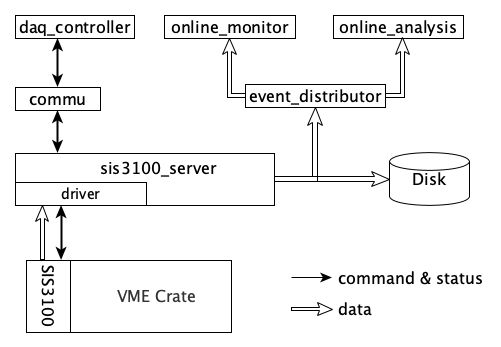
\includegraphics[width=.9\linewidth]{./koalaems_deployment.png}
\caption{\label{fig:koalaems_deployment}Design and deployment of KoalaEms}
\end{figure}
\end{document}